        \clearpage
        \begin{figure*}[ht]
            \pdfbookmark[2]{ID 01}{figure_id_01}
        	\centering
            % % 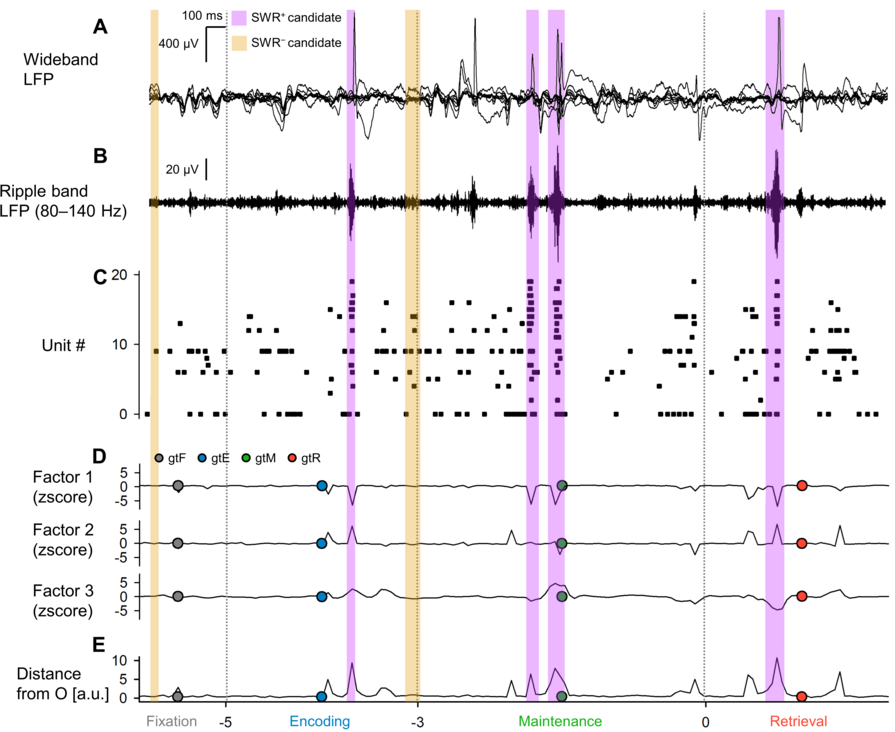
\includegraphics[width=1\textwidth]{./src/figures/.png/Figure_ID_01.png}
        	\caption{\textbf{
Local Field Potentials, Multiunit Activity, and Neural Trajectories in the Hippocampus During a Modified Sternberg Task
}
\smallskip
\\
\textbf{\textit{A.}} Representative wideband LFP signals for intracranial EEG recording from the left hippocampal head are presented. This recording took place while the subject performed a modified Sternberg working memory task. Task stages included fixation (1 s, \textit{gray}), encoding (2 s, \textit{blue}), maintenance (3 s, \textit{green}), and retrieval (2 s, \textit{red}). \textbf{\textit{B.}} Displays the associated ripple band LFP traces. Note \textit{purple} and \textit{yellow} rectangles, which denote the timings for SWR$^+$ candidates and SWR$^-$ candidates, respectively (the latter serving as control events for SWR$^+$). \textbf{\textit{C.}} A raster plot illustrates multi-unit spikes from the LFP traces. These spikes have been sorted using a spike algorithm \cite{niediek_reliable_2016}. \textbf{\textit{D.}} Shows neural trajectories (NTs) computed by GPFA\cite{yu_gaussian-process_2009} based on spike counts per unit with 50-ms bins. The geometric median of each phase is marked by dot circles. \textbf{\textit{E.}} Indicates the distance of the NT from the origin point $O$.
}
% width=1\textwidth
        	\label{fig:01}
        \end{figure*}
